% Manuscript v6 | 2026-09-28 | Final local v3 data; own VP benchmark pending.
% Tables between DATA markers are regenerated by tools/build_results.py.
\documentclass{article}
\PassOptionsToPackage{numbers,compress}{natbib}
\usepackage[final,main]{neurips_2026}
\usepackage[utf8]{inputenc}
\usepackage[T1]{fontenc}
\usepackage{amsmath,amssymb,booktabs,graphicx,microtype,url}
\usepackage{algorithm,algpseudocode}
\usepackage{xcolor,tikz}
\usetikzlibrary{arrows.meta,positioning}
\usepackage{hyperref}
\hypersetup{hidelinks,pdftitle={BDG: Batch-Dispersion Guidance for Property-Band Generation},pdfsubject={Manuscript v6, 28 September 2026}}
\newcommand{\pend}{\textsf{P}}
\newcommand{\Fbar}{\bar F}
\newcommand{\Vb}{V_b}
\newcommand{\weff}{w_{\mathrm{eff}}}
\newcommand{\IB}{\mathrm{IB}}
\newcommand{\sg}{\operatorname{stopgrad}}
\title{BDG: Batch-Dispersion Guidance for\\Property-Band Generation}
\author{Bobo Li, Henry Huang, Idea Idehpour, Haimo Fang\\
Department of Computer and Information Science, University of Pennsylvania\\
\small Manuscript v6 \quad 28 September 2026}
\begin{document}
% MAIN_TEXT_START
\maketitle
\begin{abstract}
Property-targeted generation requires samples within a tolerance band while preserving sample quality. Standard gradient guidance couples movement toward a target with contraction of the generated property distribution. We introduce Batch-Dispersion Guidance (BDG), which adjusts the deviation coefficient using the discrepancy between predicted endpoint variance and a specified variance. The target-centering coefficient remains unchanged, and the update requires the same neural calls as plug-in guidance. We study QM9 molecules in Euclidean coordinates and DeepFlyBrain DNA sequences on a probability simplex. Flow matching is the development backbone; the benchmark of our trained variance-preserving diffusion model is pending. On our flow model, plug-in guidance increases decoded coverage by 2.75 percentage points for dipole moment and 2.35 for energy gap, with reduced molecular stability. Across two molecular flow backbones, neither registered BDG setting improves coverage over plug-in at the protocol threshold; one setting incurs three losses. A gain--setpoint ablation nevertheless produces wider or narrower property distributions at fixed nominal strength. On DNA, the contracting setting increases CpG coverage over plug-in by 4.82 and 16.83 points at strengths one and four, respectively, with increased sequence-distribution mismatch. Comparisons include four recent guidance adaptations, although three collapse numerically on DNA. These results support property-dependent transfer of dispersion adjustment, without establishing a general quality advantage, exact variance regulation, or the necessity of feedback.
\end{abstract}

\section{Introduction}
Diffusion reverses corruption; flow matching learns a transport velocity \citep{karras2022elucidating,lipman2022flow}. Both generate structured samples from noise, but their quality and sampling cost require a matched comparison \citep{albergo2025stochastic}.

Gradient guidance couples target centering and spread \citep{chung2023dps,song2023lgd}. Motivated by batch interactions and moment constraints \citep{corso2024particle,mgd2026moment}, we ask whether endpoint-dispersion adjustment improves band coverage without excessive quality loss.

We study QM9 molecules and DeepFlyBrain DNA with linear flow matching and a trained VP baseline awaiting evaluation. Our hypothesis is that BDG changes spread at fixed guidance strength and improves coverage across state spaces. Our contributions are summarized as follows.
\begin{itemize}
\item We evaluate guidance on three molecular generators.
\item We derive BDG's plug-in reduction and repulsion condition.
\item We test gain and setpoint in 612 molecular ablation cells.
\item We compare recent guidance adaptations and quantify DNA transfer.
\end{itemize}

\section{Related Work}
\textbf{Continuous generation.} Flow matching fits path velocities; diffusion learns a reverse corruption process \citep{lipman2022flow,karras2022elucidating}. Stochastic interpolants connect these constructions \citep{albergo2025stochastic}.

\textbf{Dispersion and guidance.} Particle Guidance introduces batch interactions \citep{corso2024particle}; Moment Guided Diffusion imposes moment constraints \citep{mgd2026moment}; variance tilting favors feature spread \citep{vtd2026variance}. BDG contributes a scalar endpoint-variance residual inside property guidance, without their distributional guarantees.

\textbf{Molecules.} Equivariant diffusion and EquiFM model molecular geometry \citep{hoogeboom2022equivariant,song2023equifm}. We compare DPS-style plug-in, TMPD-inspired guidance, LGD-MC and TFG adaptations on common frozen backbones \citep{chung2023dps,boys2024tmpd,song2023lgd,ye2024tfg}.

\textbf{Sequences.} Dirichlet FM and Fisher Flow model simplex-valued sequences; MOG-DFM guides discrete biological sequences \citep{stark2024dirichlet,davis2024fisher,chen2025multi}. Our measured sequence comparators are ports of the guidance rules above, not reproductions of these three generators.

\section{Methods}
\subsection{Modalities, Data, and Preprocessing}\label{sec:data}
QM9 \citep{ramakrishnan2014qm9} uses centered coordinates and one-hot H/C/N/O/F types. Generator/guide $f_A$ and evaluator $f_B$ use disjoint halves of 51,527 molecules; validation/test contain 17,748/13,083. Targets are dipole $\mu$, polarizability $\alpha$, and HOMO--LUMO gap. DeepFlyBrain's 500-bp DNA occupies $(\Delta^3)^{500}$, a different state space, with 83,722/10,505/10,434 train/validation/test examples. Generators take no property input; molecules condition only on atom-count mask $M$ (Appendix~\ref{app:data}).

\subsection{Continuous Flow Matching Baseline}\label{sec:fm}
With Gaussian source $x_0$, data $x_1$ and uniform $t\in[0,1]$, we train
\begin{equation}
x_t=(1-t)x_0+tx_1,\qquad \mathcal L_{\rm FM}=\mathbb E\|v_\theta(x_t,t;M)-(x_1-x_0)\|_M^2.
\label{eq:fm}
\end{equation}
The 3.75M-parameter EGNN has eight layers of width 256. Training uses Adam, batch 256, initial rate $2\times10^{-4}$, cosine decay and EMA 0.9999. We evaluate epoch-1500 EMA weights with 100 Euler steps (Table~\ref{tab:training}).

\subsection{Diffusion Baseline}\label{sec:diff}
Our trained VP model uses the same representation and EGNN configuration. For corruption time $u$, $a(u)=\exp[-(0.1u+9.95u^2)/2]$ and $\sigma^2(u)=1-a^2(u)$:
\begin{equation}
x_u=a(u)x_1+\sigma(u)\epsilon,\qquad\mathcal L_{\rm VP}=\mathbb E\|\epsilon_\phi(x_u,u;M)-\epsilon\|_M^2.
\label{eq:vp}
\end{equation}
Sampling integrates $\mathrm dx/\mathrm du=-\frac12\beta(u)(x-\epsilon_\phi/\sigma)$ backward, with $\beta(u)=0.1+19.9u$, 100 steps and terminal denoising. Final benchmark statistics remain pending.

\subsection{Guided Generation}\label{sec:guidance}
The frozen guide evaluates $F_i=f_A(m_i)$ at $m_i=x_t^{(i)}+(1-t)v_\theta(x_t^{(i)},t;M)$. Let $s$ be the calibration-pool property standard deviation. For target $y$, plug-in guidance adds
\begin{equation}
G_i=\frac{y-F_i}{s^2}\nabla_{x_t^{(i)}}F_i,\qquad
C_i=\operatorname{clip}_{\|v_i\|}\!\left[w\frac{1-t}{\max(t,\varepsilon)}G_i\right].
\label{eq:plug}
\end{equation}
We apply $C_i$ for $t\ge0.5$, then mask and recenter molecular coordinates. The derivative includes the generator's endpoint Jacobian. All model weights stay frozen.

\subsection{Proposed Innovation: Batch-Dispersion Guidance}\label{sec:bdg}
For batch size $B$, set $\Fbar=B^{-1}\sum_iF_i$, $\Vb=(B-1)^{-1}\sum_i(F_i-\Fbar)^2$, and $\tau=\tau_m s$. BDG replaces $y-F_i$ by
\begin{equation}
\begin{aligned}
n_i&=(y-F_i)-\eta e(F_i-\Fbar)=(y-\Fbar)-\weff(F_i-\Fbar),\\
e&=(\Vb-\tau^2)/\tau^2,\qquad \weff=1+\eta e.
\end{aligned}\label{eq:bdg}
\end{equation}
The centering coefficient is preserved, but heterogeneous gradients prevent a guarantee about mean motion. Coefficients are detached before the pullback. At $\eta=0$, BDG equals plug-in. Negative $e$ weakens contraction; net repulsion requires $\weff<0$ and $\eta>1$. The setpoint does not guarantee terminal variance. Gain, setpoint and zero-gain controls test the change; isolating feedback additionally requires an unrun replay (Algorithm~\ref{alg:bdg}).

\subsection{Transfer to Modality 2}\label{sec:transfer}
A ten-layer, width-128 CNN learns a Dirichlet$(1,1,1,1)$-to-one-hot linear path. Training ran 1,500 epochs; validation selected epoch 1,450. BDG uses analytic soft GC/CpG properties. Euler steps clamp and renormalize; final decoding uses $\arg\max$ (Appendix~\ref{app:m2}).

\subsection{Model Overview}\label{sec:overview}
Figure~\ref{fig:overview} separates backbone training, frozen-model guidance and cross-modality transfer.
\begin{figure}[!t]
\centering
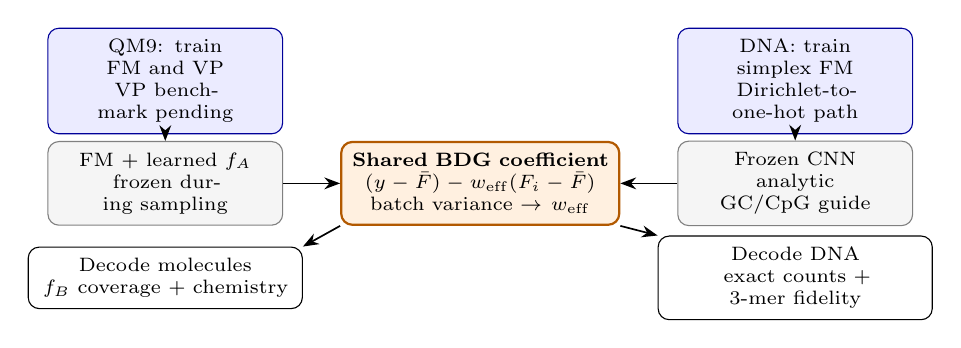
\begin{tikzpicture}[font=\scriptsize,
box/.style={draw,rounded corners,align=center,inner sep=4pt},
train/.style={box,fill=blue!8,draw=blue!60!black},
frozen/.style={box,fill=black!4,draw=black!50},
new/.style={box,fill=orange!12,draw=orange!70!black,thick},
arr/.style={-{Stealth},semithick}]
\node[train,text width=2.7cm] (fm) at (0,1.3) {QM9: train FM and VP\\VP benchmark pending};
\node[frozen,text width=2.7cm] (frozen) at (0,0) {FM + learned $f_A$\\frozen during sampling};
\node[new,text width=3.25cm] (bdg) at (4,0) {\textbf{Shared BDG coefficient}\\$(y-\Fbar)-\weff(F_i-\Fbar)$\\batch variance $\rightarrow\weff$};
\node[train,text width=2.7cm] (seq) at (8,1.3) {DNA: train simplex FM\\Dirichlet-to-one-hot path};
\node[frozen,text width=2.7cm] (sf) at (8,0) {Frozen CNN\\analytic GC/CpG guide};
\node[box,text width=3.2cm] (eval1) at (0,-1.2) {Decode molecules\\$f_B$ coverage + chemistry};
\node[box,text width=3.2cm] (eval2) at (8,-1.2) {Decode DNA\\exact counts + 3-mer fidelity};
\draw[arr] (fm)--(frozen); \draw[arr] (seq)--(sf);
\draw[arr] (frozen)--(bdg); \draw[arr] (sf)--(bdg);
\draw[arr] (bdg.south west)--(eval1.north east); \draw[arr] (bdg.south east)--(eval2.north west);
\end{tikzpicture}
\caption{Study overview: training (blue), frozen components (gray), and shared innovation (orange). Pretrained EquiFM/EDMsecond are evaluated separately; VP selection awaits its benchmark.}
\label{fig:overview}
\end{figure}

\section{Results}
\subsection{Evaluation Protocol}\label{sec:protocol}
\subsubsection{Metrics}
Targets are training medians (q50). Molecular IB counts decoded samples within $\delta=2\operatorname{MAE}_{\rm cal}(f_B)$ of $y$, accompanied by stability, validity and distinct-valid yield. DNA counts exact GC/CpG with half-widths 0.008833/0.008818, plus 3-mer JSD and Hamming diversity. Coverage comparisons stay within matched tasks.
\subsubsection{Fair Comparison and Computational Budget}
Settings use three seeds, 2,000 samples each, batches of 500 and 100 Euler steps. Headline BDG uses $\eta=4$, $w=1$; ablations and DNA also use $w=4$. Equal $w$ does not equalize force. Molecular/sequence cells sum to 81.11/5.26 wall-clock hours including evaluation (Appendix~\ref{app:evaluation}).
\subsubsection{Statistical Reporting}
Tables show mean $\pm$ seed sd. We retain the molecular protocol's unpaired binomial approximation at $|z|\ge2.99$ (18 contrasts, two-sided family level 0.05). It ignores batch coupling and rerun noise. DNA contrasts are exploratory; the gains below also survive $z=3.16$ for 32 contrasts. Unresolved differences are not equivalence claims (Table~\ref{tab:contrasts}).

\subsection{Modality 1: Flow Matching versus Diffusion}\label{sec:fmvd}
Table~\ref{tab:fmvd} reserves the VP benchmark. FM supports an explicit endpoint estimate; its selection is provisional until the trained-model comparison is complete.
% BEGIN DATA BASE
\begin{table}[!htbp]
\centering\small
\caption{Unguided QM9: percent mean $\pm$ seed sd, $3\times2{,}000$ samples. P: own VP benchmark pending. External training/architectures differ. RTX A6000 timing includes scoring.}
\label{tab:fmvd}
\begin{tabular}{lccccc}
\toprule
Generator & Mol. stable$\uparrow$ & Valid$\uparrow$ & Unique$\uparrow$ & NFE & s/sample\\
\midrule
FM, trained here & $39.7\pm0.6$ & $75.6\pm1.1$ & 99.8 & 100 & 0.051\\
VP, trained here & \pend & \pend & \pend & 101 & \pend\\
\midrule
EquiFM, pretrained & $86.2\pm0.3$ & $93.8\pm0.6$ & 99.7 & 100 & 0.086\\
EDMsecond, pretrained & $67.2\pm1.3$ & $86.0\pm1.3$ & 99.8 & 101 & 0.087\\
\bottomrule
\end{tabular}
\end{table}
% END DATA BASE

\subsection{Modality 1: Guided versus Unguided Generation}\label{sec:guidworks}
Plug-in increased our FM's coverage from 7.83\% to 10.58\% for $\mu$ and 10.28\% to 12.63\% for gap, both above threshold (Table~\ref{tab:recent}). Stability fell by 4.08/6.15 points. The $\alpha$ gain of 1.07 points remained unresolved.

\subsection{Modality 1: Innovation Ablations}\label{sec:ablations}
We crossed $\eta\in\{1,2,4,8\}$ and $\tau_m\in\{0.5,0.75,1,1.5\}$ plus $\eta=0$ at two strengths/backbones (Table~\ref{tab:ablation}). At $\eta=8,w=1$, the larger setpoint broadened spread past unguided in all six tasks (Figure~\ref{fig:results}a); tested plug-in strengths only narrowed it. This establishes additional operating range within the grid (Figures~\ref{fig:abl-fm}--\ref{fig:abl-equifm}).
\begin{table}[!htbp]
\centering\small
\caption{Controls in the 612-cell molecular grid, evaluated after decoding. Trends do not establish feedback necessity.}
\label{tab:ablation}
\begin{tabular}{lll}
\toprule
Control & Comparison & Observation\\
\midrule
Remove residual & $\eta=0$ vs plug-in & Exact on FM; rerun noise on EquiFM\\
Change strength & $\eta=0$, $w:1\to4$ & Spread remains below unguided\\
Change setpoint & $\eta=8,w=1$, $\tau_m:0.5\to1.5$ & Narrowing changes to widening\\
Change gain & $\tau_m=1.5$, $\eta:0\to8$ & Coverage lower in all 12 grids\\
\bottomrule
\end{tabular}
\end{table}

\subsection{Modality 1: Comparison with Recent Methods}\label{sec:recent}
Across two flow backbones and three properties, $\tau_m=0.5$ gave six positive but unresolved differences over plug-in; $\tau_m=1$ gave three losses and three unresolved differences (Table~\ref{tab:recent}). TFG gained more coverage with larger stability losses. Equal-strength comparisons do not rank optimally tuned methods (Tables~\ref{tab:full-equifm}--\ref{tab:full-edm}).
% BEGIN DATA M1
\begin{table}[!htbp]
\centering\small
\caption{Our FM, $w=1$: decoded IB, percent mean $\pm$ seed sd; stability in $\mu/\alpha/\mathrm{gap}$ order. Recent-method rows are matched-backbone adaptations. Full metrics and costs: Table~\ref{tab:full-fm}. Bold identifies BDG.}
\label{tab:recent}
\begin{tabular}{lcccc}
\toprule
Method & IB $\mu\uparrow$ & IB $\alpha\uparrow$ & IB gap$\uparrow$ & Mol. stable$\uparrow$\\
\midrule
Unguided & $7.8\pm0.1$ & $5.0\pm0.3$ & $10.3\pm1.0$ & 39.7 / 39.7 / 39.7\\
DPS-style plug-in & $10.6\pm0.4$ & $6.1\pm0.3$ & $12.6\pm0.7$ & 35.6 / 37.2 / 33.6\\
TMPD-inspired & $9.0\pm0.6$ & $6.1\pm0.4$ & $11.6\pm0.9$ & 38.4 / 38.9 / 37.3\\
LGD-MC & $9.6\pm0.8$ & $5.2\pm0.4$ & $10.8\pm0.7$ & 39.9 / 39.2 / 39.5\\
TFG & $28.8\pm1.6$ & $10.5\pm0.3$ & $27.5\pm0.3$ & 24.5 / 26.8 / 14.4\\
\textbf{BDG, $\tau_m=0.5$} & $11.2\pm1.1$ & $7.0\pm0.5$ & $14.2\pm0.8$ & 35.1 / 36.4 / 30.0\\
\textbf{BDG, $\tau_m=1$} & $8.9\pm0.2$ & $5.6\pm0.5$ & $10.6\pm0.2$ & 40.5 / 37.9 / 37.6\\
\bottomrule
\end{tabular}
\end{table}
% END DATA M1

\subsection{Modality 2: Transfer of the Innovation}\label{sec:m2}
At $w=4$, BDG with $\tau_m=0.5$ increased GC/CpG coverage over plug-in by 2.32/16.83 points, while increasing JSD (Table~\ref{tab:m2}). At $w=1$, gains were 0.42/4.82 points; only CpG cleared the exploratory threshold. The $\tau_m=1$ setting improved neither property. Plug-in, TMPD and LGD-MC coincide numerically because endpoint uncertainty nearly vanishes in this window. They are three implemented adaptations but one effective comparator.
% BEGIN DATA M2
\begin{table}[!htbp]
\centering\small
\caption{DNA, $w=4$, $t\ge0.5$: decoded IB (percent mean $\pm$ seed sd); 3-mer JSD ($\times10^{-4}$, GC/CpG). All fidelity values match the strength. TFG-MC is a restricted adaptation. Other metrics/strength: Table~\ref{tab:full-m2}.}
\label{tab:m2}
\begin{tabular}{lccc}
\toprule
Method & GC IB$\uparrow$ & CpG IB$\uparrow$ & JSD$\downarrow$\\
\midrule
Unguided & $14.0\pm1.0$ & $50.2\pm1.6$ & 4.53 / 4.53\\
DPS-style plug-in & $14.1\pm1.0$ & $51.6\pm1.4$ & 4.61 / 4.63\\
TMPD-inspired & $14.1\pm1.0$ & $51.6\pm1.4$ & 4.61 / 4.63\\
LGD-MC & $14.1\pm1.0$ & $51.6\pm1.4$ & 4.61 / 4.63\\
TFG-MC adaptation & $14.1\pm1.0$ & $51.1\pm1.7$ & 4.59 / 4.58\\
\textbf{BDG, $\tau_m=0.5$} & $16.4\pm1.2$ & $68.5\pm1.2$ & 5.93 / 7.73\\
\textbf{BDG, $\tau_m=1$} & $14.1\pm1.0$ & $50.3\pm1.5$ & 4.54 / 4.52\\
\bottomrule
\end{tabular}
\end{table}
% END DATA M2
\begin{figure}[!t]
\centering
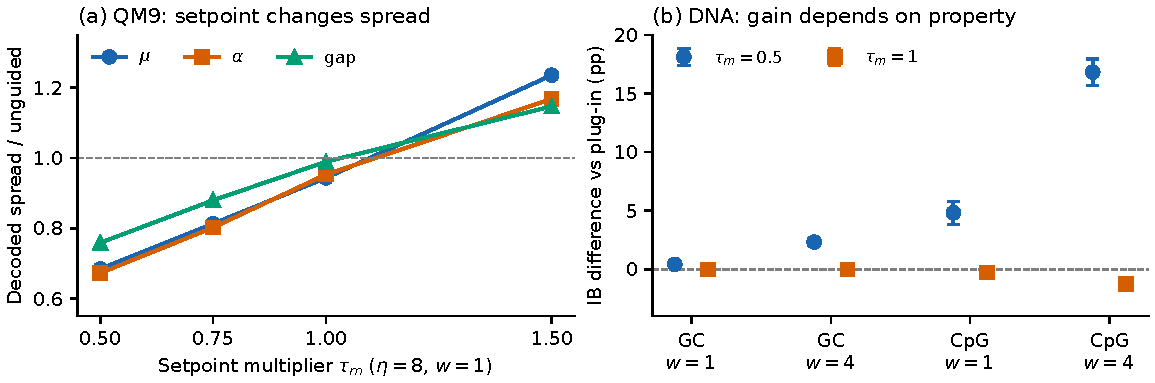
\includegraphics[width=\linewidth]{figs/results_v6.pdf}
\caption{Final-run measurements. (a) Our FM, decoded property standard deviation relative to unguided; points pool three seeds. (b) BDG minus plug-in on DNA, $\eta=4$, window $t\ge0.5$; bars show sd of three paired seed differences, not confidence intervals. Coverage scales differ by property.}
\label{fig:results}
\end{figure}

\subsection{Cross-Modality Analysis and Failure Modes}\label{sec:failure}
Molecular BDG gains remain unresolved; CpG gains pass the exploratory threshold. Strong corrections reduce chemistry or sequence fidelity. On GC alone, early guidance added 22.82 points for plug-in, versus the best late-window gain of 4.23 over unguided; clipping confounds this diagnostic. Property spread does not establish functional diversity.

\section{Discussion}
The molecular experiments support controllability with quality costs, without a resolved BDG improvement over plug-in. DNA transfer is positive for the contracting CpG setting and weaker for GC. The trained FM--VP comparison remains pending.

BDG changes the deviation coefficient while retaining the scalar centering coefficient. The ablations connect the setpoint to spread; heterogeneous gradients, clipping and decoding explain why this algebra does not guarantee better target coverage. Fixed nominal strength does not isolate feedback from increased force.

A matched-force replay and batch-aware intervals would sharpen attribution. Joint in-band-and-stable yield requires sample-level data; composition fidelity does not establish enhancer function. The supported claim is that one dispersion rule transfers across state spaces, with benefits that depend on the property and operating regime.
% MAIN_TEXT_END
\clearpage
\bibliographystyle{ieeetr}
\bibliography{citation,refs_extra}
\clearpage
\appendix
\renewcommand{\thetable}{S\arabic{table}}
\renewcommand{\theHtable}{S\arabic{table}}
\setcounter{table}{0}
\renewcommand{\thefigure}{S\arabic{figure}}
\renewcommand{\theHfigure}{S\arabic{figure}}
\setcounter{figure}{0}
\section{Reproducibility and Extended Results}
\subsection{Data Sources and Splits}\label{app:data}
QM9 uses the DeepChem/MoleculeNet packaging. The project retains the 3,054 entries excluded as uncharacterized in common EDM preprocessing, so published EDM dataset definitions are not identical. A seeded permutation creates the four splits stated in Section~\ref{sec:data}. Coordinates are centered, padded atoms are masked, and coordinates and one-hot features have no additional scaling. The E(3)-equivariant generator handles rotation and translation; invariant property predictors use training-derived normalization. Sizes and initial noise are shared across arms within each backend and seed. No property label enters either generator.

DeepFlyBrain is the 500-bp enhancer data used by Dirichlet FM \citep{stark2024dirichlet}. Four ambiguous training examples were excluded from the supplied 83,726. The retained splits are 83,722/10,505/10,434; channels are A/C/G/T. Class labels are unused by our unconditional generator. These random-example splits do not test sequence-cluster generalization. The older 200-bp experiment is excluded.

Exact targets and calibration values are preserved in each source cell. Molecular band half-widths for our predictor pair are 0.17541 D for $\mu$, 0.50618 Bohr$^3$ for $\alpha$, and 0.00748 Ha for gap. External EquiFM uses a different predictor pair and therefore different acceptance widths. Its coverage must not be ranked directly against our FM's coverage.

\subsection{Training and Checkpoint Records}\label{app:training}
Table~\ref{tab:training} distinguishes measured checkpoint records from the VP configuration. For coordinates $c$, features $f$ and broadcast mask $M$, the training norm is
\[
\|z\|_M^2=\frac{\|M\odot z^c\|_2^2}{3\sum M}+\frac{\|M\odot z^f\|_2^2}{5\sum M}.
\]
Gaussian coordinate noise is centered; feature noise is independent Gaussian. The molecular FM checkpoint records epoch 1500, EMA, and the hyperparameters below. The training code selects validation atom stability with validation loss as a tie-breaker, but the evaluated FM export is the recorded final-epoch EMA. The pending VP benchmark must disclose its actual selected checkpoint before a matched model-selection claim is made. VP training samples $u\in[10^{-3},1]$; its probability-flow ODE follows Equation~\eqref{eq:vp}.

\begin{table}[!htbp]
\centering\small
\caption{Training records. VP settings are configured; its final benchmark/provenance is pending. Molecular predictors use one network per property and training half. Unrecorded training time is not inferred from sampling time.}
\label{tab:training}
\begin{tabular}{llll}
\toprule
Setting & Molecular FM / VP & $f_A$ / $f_B$ & Sequence FM\\
\midrule
Architecture & EGNN, 256, 8 layers & EGNN, 128, 4 & CNN, 128, 10\\
Parameters & 3.75M / 3.75M configured & 429,825 each & approximately 1.02M\\
Training data & \texttt{train\_a} & \texttt{train\_a}/\texttt{train\_b} & 83,722 sequences\\
Objective & velocity / noise MSE & property MSE & velocity MSE\\
Epochs & 1500 / 1500 configured & 120 & 1500 completed\\
Selected weights & epoch-1500 EMA / pending & validation checkpoint & epoch 1450\\
Batch size & 256 & 128 & 256\\
Optimizer & Adam & Adam & Adam\\
Initial learning rate & $2\times10^{-4}$ & $3\times10^{-4}$ & $2\times10^{-3}$\\
Schedule & cosine, floor 5\% & cosine & cosine to zero\\
EMA & 0.9999 & none & none\\
Training seed & 20260918 / configured & 20260918 & 20260921\\
Training time & not fully recorded & not fully recorded & 539.7 min\\
\bottomrule
\end{tabular}
\end{table}

Sequence training performed 492,000 updates across 1,500 epochs. Validation selected update 475,600 (epoch 1450), loss 0.0633644, with 121.75M sample-views at the selected checkpoint. The total run lasted 539.7 minutes on RTX A6000, including validation. We distinguish completed training length from the selected checkpoint's age. The checkpoint uses Adam without EMA; its best-validation weights are sampled.

\begin{table}[!htbp]
\centering\small
\caption{Checkpoint fingerprints from the result records and local files. Prefixes identify artifacts; full hashes are retained in the source records.}
\label{tab:hashes}
\begin{tabular}{lll}
\toprule
Component & Identifier & Evidence\\
\midrule
Our molecular FM & MD5 \texttt{e19ccc06} & v3 cells, epoch 1500\\
Borrowed EDMsecond & MD5 \texttt{6abbd010} & v3 cells, released checkpoint\\
Sequence FM & MD5 \texttt{7f59b60b} & local checkpoint, best validation\\
Our VP & pending benchmark & no result row substituted\\
\bottomrule
\end{tabular}
\end{table}
Table~\ref{tab:hashes} identifies the evaluated artifacts. The molecular cells record PyTorch 2.11.0+cu130, CUDA 13.0 and RTX A6000. The sequence training report identifies RTX A6000, but individual sequence evaluation cells omit the device; those timings are not treated as hardware-matched cross-modality benchmarks.

\subsection{Evaluation, Uncertainty, and Cost}\label{app:evaluation}
Molecular seeds are 20261001, 20261002 and 20261003. Sequence seeds are 20260921, 20260922 and 20260923. Each 2,000-sample cell contains four independent controller batches of size 500. Enlarging the total sample count adds batches, not observations to a single variance estimate. At fixed weights, seed variation measures sampling variation, not training uncertainty.

Molecular coverage counts decoded samples satisfying $|f_B(\hat x)-y|\le\delta$. Calibration uses 3,000 molecules drawn from the two training halves; each internal predictor is scored on the half it did not train on. The wrapper sets $s$ to the property standard deviation of this calibration pool, which differs from the raw predictor checkpoint's normalization scale. This $s$ sets the guidance energy and BDG setpoint; evaluator error sets $\delta$. Coverage on continuous features remains in source records but is not substituted for decoded IB.

Atom stability checks bond/valence rules; molecular stability requires every atom to pass. RDKit validity checks reconstruction and sanitization. Uniqueness divides distinct valid SMILES by valid samples; distinct-valid yield divides by all attempts. None is an energy or experimental viability measurement. IB includes invalid molecules, so usable yield requires the joint event of decoded in-band membership and stability. Marginal IB and stability cannot be multiplied to recover that event. The local aggregate results do not include the sample-level sidecars needed for this joint analysis.

The reported unpaired statistic is
\[
 z=\frac{p_a-p_b}{\sqrt{p_a(1-p_a)/6000+p_b(1-p_b)/6000}}.
\]
The registered molecular bar is 2.99. Table~\ref{tab:contrasts} reports the corresponding threshold-sized difference separately for every contrast; it is neither a power calculation nor evidence of equivalence. Within-batch dependence can invalidate an independent-Bernoulli variance, and common-noise pairing changes covariance. We retain this protocol statistic with explicit limitations and show seed standard deviations. A batch-aware paired bootstrap would need the sample-level records. The decoded analysis uses the same registered rule as the protocol's continuous metric; both yield the same headline BDG verdict counts. DNA uses the rule only as an exploratory comparison, and the stated positive effects survive the 32-contrast threshold of 3.16. For selections from the full molecular grid, the protocol's adjusted bar is 3.49; the paper makes descriptive grid claims without converting them into headline tests.

EquiFM same-seed reruns differ by up to 0.007 in continuous coverage. Its $\eta=0$ control agrees with plug-in only to the rerun tolerance, not bitwise. Our FM reproduces exactly. EDMsecond has same-seed variation up to 0.0015 in molecular stability. Neither binomial errors nor three seed values fully characterize this extra implementation variability.

The molecular run contains 144 headline and 612 ablation cells. Summed recorded wall-clock is 15.96 hours for headline and 65.15 for ablations, 81.11 total. The DNA files contain 84 headline, 111 ablation/window and four single-seed strength cells, with 12 repeated configurations across trees; the 199 files represent 187 distinct cells and 5.26 hours of recorded compute. The repeated configurations are checked for agreement and never pooled as extra seeds. Concurrent cells and evaluation overhead prevent interpreting these totals as elapsed time or accelerator utilization.

NFE counts solver field evaluations, distinct from generator forwards and derivative calls. For each molecular batch, plug-in and BDG record 200 generator forwards, 50 generator VJPs, and 50 guide forward/backward pairs; unguided records 100 generator forwards. Sequence guided batches record 150 generator forwards and 50 VJPs. BDG adds scalar reductions to plug-in, not another neural call. Equal calls do not imply equal measured runtime. Clip fractions divide clipped sample-steps by samples times guided steps \emph{per batch}; using the batch-summed step count understates them fourfold.

\subsection{Full Molecular Comparisons}\label{app:comparisons}
Tables~\ref{tab:full-fm}, \ref{tab:full-equifm} and~\ref{tab:full-edm} report every headline arm and property. All numbers are generated by this project; no published score is mixed into these rows. EquiFM uses the released TFG guide/evaluator pair; our FM and borrowed EDMsecond use our disjoint pair. External training overlap, architectures, scales and selection differ, so all guidance contrasts stay within a backend.

DPS-style plug-in adapts posterior guidance to a Gaussian property energy and a flow endpoint. TMPD-inspired guidance uses a linearized uncertainty correction; LGD-MC marginalizes a local property loss; TFG combines training-free corrections. The implementations retain the local endpoint, clipping and timing choices in the cell records, and are adaptations of the cited methods, not reproductions of every original experimental setting. Molecular TFG and sequence TFG-MC are different implementations; the latter omits full TFG's iterative schedule.
% BEGIN DATA FULL-FM
\begin{table}[!htbp]
\centering\small
\caption{Full our FM headline evaluation. IB is decoded; IB and stability show percent mean $\pm$ seed sd. Validity and distinct-valid yield (DV) are percentages; time is recorded cell wall-clock divided by attempts. $w=1$, $t\ge0.5$, three seeds, $n=2{,}000$ each.}
\label{tab:full-fm}
\begin{tabular}{llccccc}
\toprule
Property & Method & IB$\uparrow$ & Stable$\uparrow$ & Valid$\uparrow$ & DV$\uparrow$ & s/sample\\
\midrule
$\mu$ & Unguided & $7.8\pm0.1$ & $39.7\pm0.6$ & 75.6 & 75.5 & 0.051\\
$\mu$ & DPS-style plug-in & $10.6\pm0.4$ & $35.6\pm0.3$ & 72.5 & 72.4 & 0.119\\
$\mu$ & TMPD-inspired & $9.0\pm0.6$ & $38.4\pm0.6$ & 74.8 & 74.7 & 0.255\\
$\mu$ & LGD-MC & $9.6\pm0.8$ & $39.9\pm0.3$ & 75.5 & 75.4 & 0.229\\
$\mu$ & TFG & $28.8\pm1.6$ & $24.5\pm1.0$ & 62.8 & 62.7 & 0.122\\
$\mu$ & \textbf{BDG, $\tau_m=0.5$} & $11.2\pm1.1$ & $35.1\pm1.1$ & 71.4 & 71.2 & 0.119\\
$\mu$ & \textbf{BDG, $\tau_m=1$} & $8.9\pm0.2$ & $40.5\pm0.8$ & 76.5 & 76.3 & 0.119\\
\midrule
$\alpha$ & Unguided & $5.0\pm0.3$ & $39.7\pm0.6$ & 75.6 & 75.5 & 0.050\\
$\alpha$ & DPS-style plug-in & $6.1\pm0.3$ & $37.2\pm1.6$ & 73.7 & 73.6 & 0.118\\
$\alpha$ & TMPD-inspired & $6.1\pm0.4$ & $38.9\pm1.1$ & 75.1 & 75.0 & 0.200\\
$\alpha$ & LGD-MC & $5.2\pm0.4$ & $39.2\pm1.3$ & 74.9 & 74.9 & 0.224\\
$\alpha$ & TFG & $10.5\pm0.3$ & $26.8\pm0.8$ & 61.2 & 61.1 & 0.121\\
$\alpha$ & \textbf{BDG, $\tau_m=0.5$} & $7.0\pm0.5$ & $36.4\pm1.0$ & 72.2 & 72.1 & 0.118\\
$\alpha$ & \textbf{BDG, $\tau_m=1$} & $5.6\pm0.5$ & $37.9\pm1.1$ & 75.1 & 75.1 & 0.118\\
\midrule
gap & Unguided & $10.3\pm1.0$ & $39.7\pm0.6$ & 75.6 & 75.5 & 0.051\\
gap & DPS-style plug-in & $12.6\pm0.7$ & $33.6\pm0.8$ & 69.9 & 69.8 & 0.119\\
gap & TMPD-inspired & $11.6\pm0.9$ & $37.3\pm0.7$ & 73.8 & 73.7 & 0.201\\
gap & LGD-MC & $10.8\pm0.7$ & $39.5\pm0.8$ & 75.2 & 75.1 & 0.225\\
gap & TFG & $27.5\pm0.3$ & $14.4\pm0.8$ & 45.5 & 45.5 & 0.122\\
gap & \textbf{BDG, $\tau_m=0.5$} & $14.2\pm0.8$ & $30.0\pm0.4$ & 65.8 & 65.7 & 0.119\\
gap & \textbf{BDG, $\tau_m=1$} & $10.6\pm0.2$ & $37.6\pm0.8$ & 74.3 & 74.2 & 0.119\\
\bottomrule
\end{tabular}
\end{table}
% END DATA FULL-FM
\clearpage
% BEGIN DATA FULL-EQUIFM
\begin{table}[!htbp]
\centering\small
\caption{Full borrowed EquiFM headline evaluation. IB is decoded; IB and stability show percent mean $\pm$ seed sd. Validity and distinct-valid yield (DV) are percentages; time is recorded cell wall-clock divided by attempts. $w=1$, $t\ge0.5$, three seeds, $n=2{,}000$ each.}
\label{tab:full-equifm}
\begin{tabular}{llccccc}
\toprule
Property & Method & IB$\uparrow$ & Stable$\uparrow$ & Valid$\uparrow$ & DV$\uparrow$ & s/sample\\
\midrule
$\mu$ & Unguided & $8.7\pm0.8$ & $86.2\pm0.3$ & 93.8 & 93.5 & 0.086\\
$\mu$ & DPS-style plug-in & $10.9\pm0.9$ & $82.1\pm0.7$ & 91.9 & 91.6 & 0.231\\
$\mu$ & TMPD-inspired & $9.0\pm0.3$ & $85.3\pm0.4$ & 93.5 & 93.2 & 0.366\\
$\mu$ & LGD-MC & $9.7\pm0.3$ & $85.5\pm0.4$ & 93.3 & 93.1 & 0.474\\
$\mu$ & TFG & $11.9\pm0.3$ & $74.0\pm0.7$ & 86.5 & 86.2 & 0.301\\
$\mu$ & \textbf{BDG, $\tau_m=0.5$} & $12.1\pm0.5$ & $79.3\pm0.7$ & 90.9 & 90.6 & 0.232\\
$\mu$ & \textbf{BDG, $\tau_m=1$} & $8.9\pm0.7$ & $85.8\pm0.3$ & 93.6 & 93.3 & 0.232\\
\midrule
$\alpha$ & Unguided & $2.1\pm0.1$ & $86.2\pm0.3$ & 93.8 & 93.5 & 0.087\\
$\alpha$ & DPS-style plug-in & $2.1\pm0.2$ & $82.9\pm0.4$ & 91.9 & 91.7 & 0.233\\
$\alpha$ & TMPD-inspired & $2.1\pm0.3$ & $84.8\pm0.3$ & 93.3 & 93.0 & 0.368\\
$\alpha$ & LGD-MC & $2.1\pm0.1$ & $85.5\pm0.9$ & 93.3 & 93.0 & 0.476\\
$\alpha$ & TFG & $3.4\pm0.5$ & $64.5\pm0.5$ & 84.5 & 84.4 & 0.302\\
$\alpha$ & \textbf{BDG, $\tau_m=0.5$} & $2.5\pm0.2$ & $76.6\pm0.5$ & 89.5 & 89.2 & 0.233\\
$\alpha$ & \textbf{BDG, $\tau_m=1$} & $2.0\pm0.1$ & $84.8\pm0.5$ & 92.8 & 92.6 & 0.233\\
\midrule
gap & Unguided & $4.9\pm0.2$ & $86.2\pm0.3$ & 93.8 & 93.5 & 0.086\\
gap & DPS-style plug-in & $5.9\pm0.3$ & $82.7\pm0.4$ & 91.9 & 91.7 & 0.231\\
gap & TMPD-inspired & $5.1\pm0.3$ & $84.6\pm0.7$ & 92.7 & 92.4 & 0.365\\
gap & LGD-MC & $5.1\pm0.4$ & $86.1\pm0.2$ & 93.5 & 93.3 & 0.473\\
gap & TFG & $10.9\pm0.2$ & $55.5\pm1.4$ & 76.4 & 76.2 & 0.300\\
gap & \textbf{BDG, $\tau_m=0.5$} & $6.8\pm0.8$ & $77.4\pm1.1$ & 90.1 & 90.0 & 0.231\\
gap & \textbf{BDG, $\tau_m=1$} & $5.0\pm0.4$ & $85.6\pm0.3$ & 93.4 & 93.1 & 0.231\\
\bottomrule
\end{tabular}
\end{table}
% END DATA FULL-EQUIFM
% BEGIN DATA FULL-EDM
\begin{table}[!htbp]
\centering\small
\caption{Full borrowed EDMsecond headline evaluation. IB is decoded; IB and stability show percent mean $\pm$ seed sd. Validity and distinct-valid yield (DV) are percentages; time is recorded cell wall-clock divided by attempts. $w=1$, $t\ge0.5$, three seeds, $n=2{,}000$ each.}
\label{tab:full-edm}
\begin{tabular}{llccccc}
\toprule
Property & Method & IB$\uparrow$ & Stable$\uparrow$ & Valid$\uparrow$ & DV$\uparrow$ & s/sample\\
\midrule
$\mu$ & Unguided & $9.4\pm0.2$ & $67.2\pm1.3$ & 86.0 & 85.8 & 0.087\\
$\mu$ & DPS-style plug-in & $11.2\pm1.1$ & $62.2\pm0.6$ & 82.8 & 82.7 & 0.210\\
\midrule
$\alpha$ & Unguided & $5.4\pm0.7$ & $67.2\pm1.2$ & 86.0 & 85.8 & 0.087\\
$\alpha$ & DPS-style plug-in & $6.1\pm0.4$ & $64.6\pm0.8$ & 84.1 & 83.9 & 0.208\\
\midrule
gap & Unguided & $10.8\pm0.7$ & $67.1\pm1.3$ & 86.0 & 85.8 & 0.087\\
gap & DPS-style plug-in & $12.8\pm0.7$ & $57.9\pm1.7$ & 80.3 & 80.2 & 0.209\\
\bottomrule
\end{tabular}
\end{table}
% END DATA FULL-EDM
\clearpage
% BEGIN DATA CONTRASTS
\begin{table}[!htbp]
\centering\small
\caption{BDG minus plug-in on decoded molecular IB. Differences, paired seed sd and the threshold-sized difference $2.99\,\mathrm{se}(\Delta)$ are in percentage points. The registered unpaired statistic is shown separately from descriptive pairing.}
\label{tab:contrasts}
\begin{tabular}{llccccc}
\toprule
Backend & Property & $\tau_m$ & $\Delta$IB & SD$(\Delta)$ & $z$ & Threshold\\
\midrule
fm & $\mu$ & 0.5 & +0.63 & 1.45 & +1.11 & 1.70\\
fm & $\mu$ & 1 & -1.68 & 0.19 & -3.11 & 1.62\\
fm & $\alpha$ & 0.5 & +0.90 & 0.50 & +2.00 & 1.35\\
fm & $\alpha$ & 1 & -0.43 & 0.75 & -1.01 & 1.28\\
fm & gap & 0.5 & +1.52 & 0.21 & +2.44 & 1.86\\
fm & gap & 1 & -2.07 & 0.72 & -3.54 & 1.75\\
equifm & $\mu$ & 0.5 & +1.25 & 0.70 & +2.15 & 1.74\\
equifm & $\mu$ & 1 & -1.93 & 0.62 & -3.55 & 1.63\\
equifm & $\alpha$ & 0.5 & +0.45 & 0.13 & +1.65 & 0.81\\
equifm & $\alpha$ & 1 & -0.02 & 0.31 & -0.06 & 0.77\\
equifm & gap & 0.5 & +0.90 & 0.56 & +2.02 & 1.33\\
equifm & gap & 1 & -0.93 & 0.67 & -2.25 & 1.24\\
\bottomrule
\end{tabular}
\end{table}
% END DATA CONTRASTS

\subsection{Complete Molecular Ablation Grids}\label{app:ablations}
Figures~\ref{fig:abl-fm} and~\ref{fig:abl-equifm} show every nonzero gain/setpoint combination as decoded coverage change from its own zero-gain control, with strengths kept separate. Every heatmap value is recomputed from three seed cells. Increasing $\eta$ need not monotonically improve coverage at a contracting setpoint, particularly at $w=4$. The widening setpoint lowers coverage relative to zero gain in every grid. This is consistent with the trade-off between spread and occupancy of a fixed band; it does not establish a unique causal role for feedback.

At $\eta=8,w=1,\tau_m=1.5$, decoded spread exceeds unguided for all three properties and both flow backends, approximately 1.15--1.25 times the reference. The tested positive plug-in strengths $w\in\{1,4\}$ remain below it. This comparison does not exclude signed strengths, arbitrary schedules, or a shifted plug-in target from reaching similar states. One-sided residuals, open-loop replay and signed-strength controls were not part of the completed grid.
\begin{figure}[!htbp]
\centering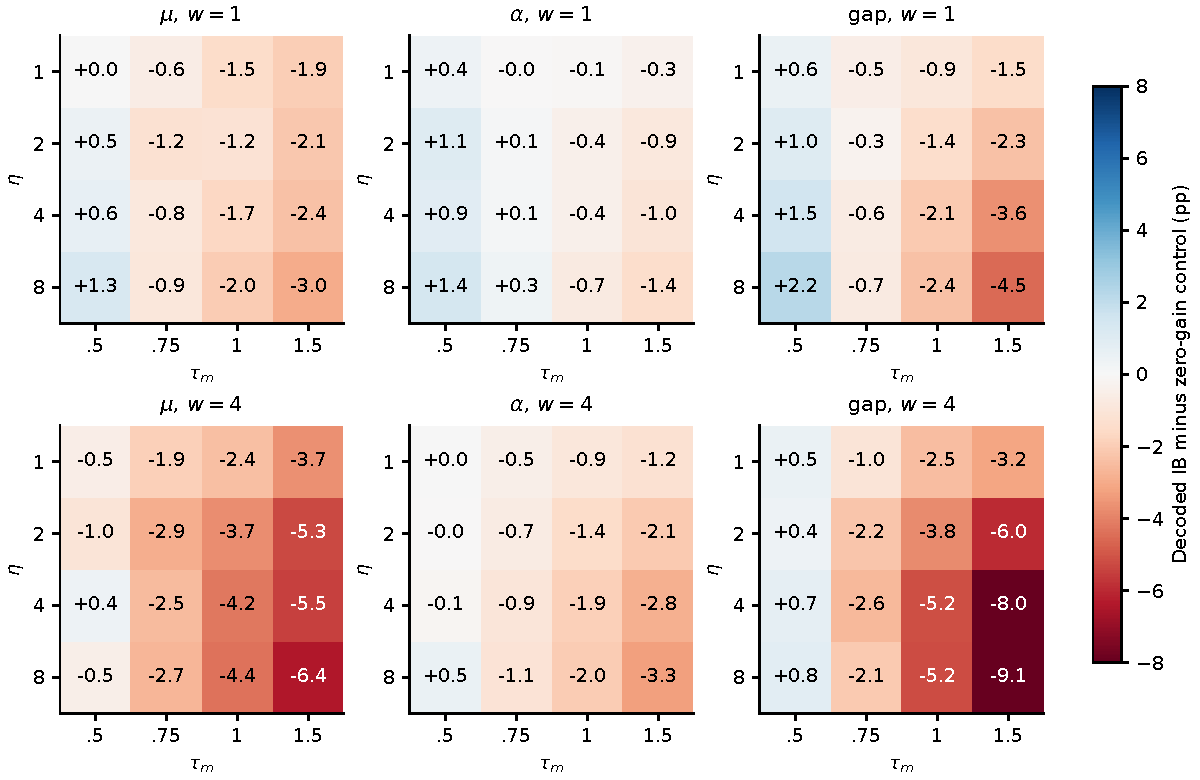
\includegraphics[width=\linewidth]{figs/ablation_fm_v6.pdf}
\caption{Our FM: full decoded coverage ablation. Each panel fixes property and strength; entries are percentage-point changes from $\eta=0$ at that strength. The color scale is shared with Figure~\ref{fig:abl-equifm}; values outside its range retain their exact text.}
\label{fig:abl-fm}
\end{figure}
\begin{figure}[!htbp]
\centering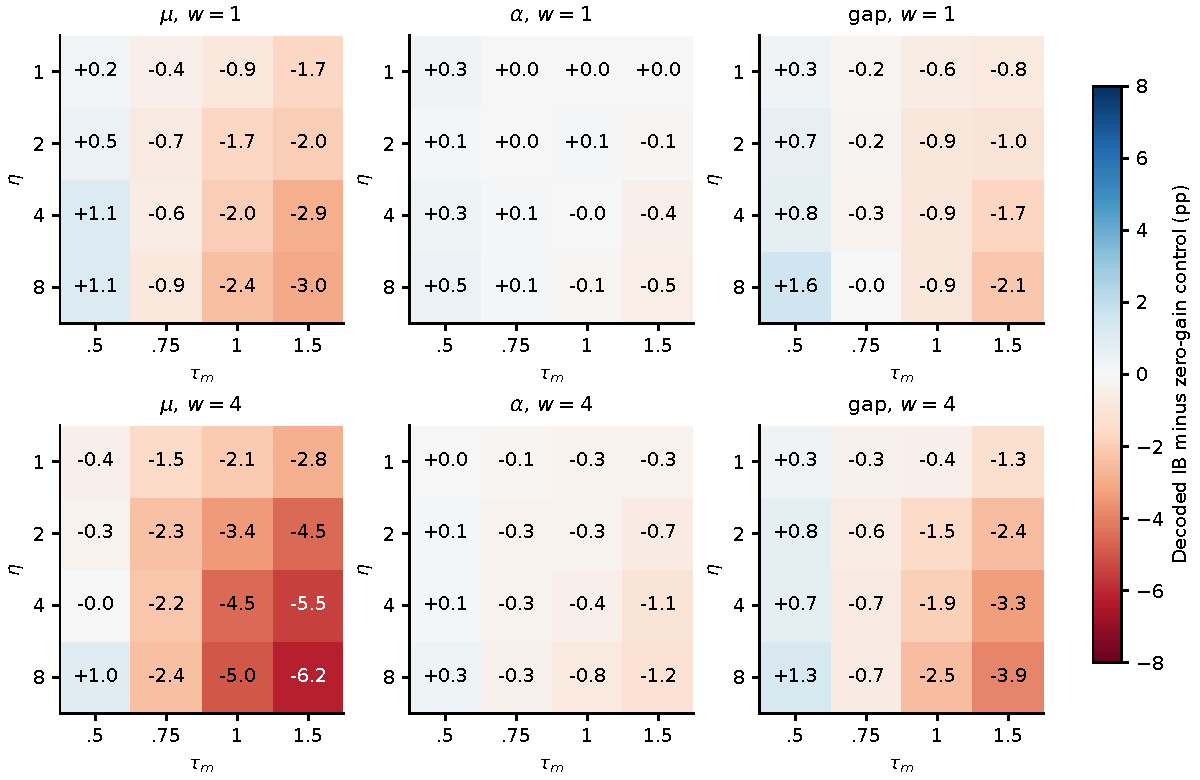
\includegraphics[width=\linewidth]{figs/ablation_equifm_v6.pdf}
\caption{Borrowed EquiFM: the same complete grid and matched zero-gain contrasts. Rerun variability accompanies the three-seed averages.}
\label{fig:abl-equifm}
\end{figure}
\clearpage

\subsection{Sequence Transfer and Failure Diagnostics}\label{app:m2}
The checkpoint joins uniform Dirichlet noise to one-hot 500-base-pair sequences. At each step, the sampler clamps negatives, normalizes each position, and decodes final samples by the largest channel. Endpoint extrapolation for guidance can leave the simplex, so soft properties and decoded counts can disagree. For relaxed sequence $p$ of length $L$,
\[
 F_{\rm GC}(p)=L^{-1}\sum_j(p_{j,C}+p_{j,G}),\qquad
 F_{\rm CpG}(p)=(L-1)^{-1}\sum_{j=1}^{L-1}p_{j,C}p_{j+1,G}.
\]
GC is affine; CpG is quadratic. The final metric counts bases or adjacent pairs after decoding. Its half-width is $\delta=\max(0.16s,4.4q)$, where the count quantum is $q=1/500$ for GC and $q=1/499$ for CpG. GC has $s=0.055206$, $\delta/s=0.160$; CpG has $s=0.014748$, $\delta/s=0.598$ because its lattice floor binds. Absolute coverage levels therefore cannot be ranked across properties or against molecular coverage.

Table~\ref{tab:full-m2} gives all recent-method adaptations, both registered BDG settings and both strengths. The 3-mer JSD reference is the training split. Hamming diversity uses the first 256 decoded sequences and all ordered pairs including self-pairs; it is almost unchanged around 0.7456 and is not evidence of functional diversity. Every fidelity number is paired with coverage at the same strength. All sequences decode to valid A/C/G/T strings, so categorical validity is uninformative here.

In the late window, plug-in, TMPD and LGD-MC differ by at most $4.2\times10^{-6}$ on the identity-check metrics. Measured endpoint uncertainty declines about 38,000-fold before $t=0.5$, suppressing the corrections that distinguish them. These ports meet a method-comparison design but supply limited independent evidence. Dirichlet FM, Fisher Flow and MOG-DFM were not evaluated under these GC/CpG bands. The current transfer benchmark must not be described as a reproduction of those sequence generators.

For GC at $w=4$, contracting BDG increases coverage while the normalized bias worsens from +0.997 to +1.231. Its clipping fraction rises to 9.24\% from plug-in's 0.079\%; CpG clipping is 7.41\% versus 0.21\%. Thus equal nominal strength does not equalize applied correction. A GC-only window diagnostic at $w=1$ increased plug-in coverage by 22.82 points when guidance began at zero. BDG at $\tau_m=0.5$ was 2.33 points below that plug-in result; $\tau_m=1$ was 20.80 points below. About a third of early-window steps clip. The ratio of window gain to the best late-window GC gain is about 5.4, and no corresponding CpG early-window result was run.

A separate frozen DeepFlyBrain predictor diagnostic exists in \path{results/m2_dfb_activity.json}. Its port was not verified numerically against the published Keras model in the committed evidence, so we do not claim published-oracle equivalence or biological function from these scores. Base composition, low-order k-mers and Hamming diversity cannot establish enhancer activity or cell-type specificity.
% BEGIN DATA FULL-M2
\begin{table}[!htbp]
\centering\small
\caption{All DNA headline settings. IB is percent mean $\pm$ seed sd; JSD is multiplied by $10^4$; Conf. is decoding confidence; Div. is normalized Hamming distance; Clip is percent of guided sample-steps. Unguided rows repeat a common reference and are never pooled twice.}
\label{tab:full-m2}
\begin{tabular}{llcccccc}
\toprule
Prop., $w$ & Method & IB$\uparrow$ & JSD$\downarrow$ & Conf. & Div. & Clip & s/seq.\\
\midrule
GC, 1 & Unguided & $14.0\pm1.0$ & 4.53 & 0.958 & 0.7456 & 0.00 & 0.021\\
GC, 1 & DPS-style plug-in & $14.0\pm0.9$ & 4.53 & 0.958 & 0.7456 & 0.00 & 0.042\\
GC, 1 & TMPD-inspired & $14.0\pm0.9$ & 4.53 & 0.958 & 0.7456 & 0.00 & 0.045\\
GC, 1 & LGD-MC & $14.0\pm0.9$ & 4.53 & 0.958 & 0.7456 & 0.00 & 0.035\\
GC, 1 & TFG-MC adaptation & $14.1\pm1.0$ & 4.53 & 0.958 & 0.7456 & 0.00 & 0.047\\
GC, 1 & \textbf{BDG, $\tau_m=0.5$} & $14.5\pm1.0$ & 4.95 & 0.956 & 0.7456 & 0.56 & 0.042\\
GC, 1 & \textbf{BDG, $\tau_m=1$} & $14.0\pm1.0$ & 4.53 & 0.958 & 0.7456 & 0.00 & 0.042\\
\midrule
GC, 4 & Unguided & $14.0\pm1.0$ & 4.53 & 0.958 & 0.7456 & 0.00 & 0.021\\
GC, 4 & DPS-style plug-in & $14.1\pm1.0$ & 4.61 & 0.958 & 0.7456 & 0.08 & 0.040\\
GC, 4 & TMPD-inspired & $14.1\pm1.0$ & 4.61 & 0.958 & 0.7456 & 0.08 & 0.051\\
GC, 4 & LGD-MC & $14.1\pm1.0$ & 4.61 & 0.958 & 0.7456 & 0.08 & 0.047\\
GC, 4 & TFG-MC adaptation & $14.1\pm1.0$ & 4.59 & 0.958 & 0.7456 & 0.06 & 0.043\\
GC, 4 & \textbf{BDG, $\tau_m=0.5$} & $16.4\pm1.2$ & 5.93 & 0.947 & 0.7457 & 9.24 & 0.028\\
GC, 4 & \textbf{BDG, $\tau_m=1$} & $14.1\pm1.0$ & 4.54 & 0.958 & 0.7456 & 0.01 & 0.028\\
\midrule
CpG, 1 & Unguided & $50.2\pm1.6$ & 4.53 & 0.958 & 0.7456 & 0.00 & 0.036\\
CpG, 1 & DPS-style plug-in & $50.5\pm1.8$ & 4.53 & 0.958 & 0.7456 & 0.02 & 0.074\\
CpG, 1 & TMPD-inspired & $50.5\pm1.8$ & 4.53 & 0.958 & 0.7456 & 0.02 & 0.120\\
CpG, 1 & LGD-MC & $50.5\pm1.8$ & 4.53 & 0.958 & 0.7456 & 0.02 & 0.102\\
CpG, 1 & TFG-MC adaptation & $50.4\pm1.7$ & 4.54 & 0.958 & 0.7456 & 0.01 & 0.089\\
CpG, 1 & \textbf{BDG, $\tau_m=0.5$} & $55.3\pm0.8$ & 5.26 & 0.956 & 0.7456 & 0.98 & 0.073\\
CpG, 1 & \textbf{BDG, $\tau_m=1$} & $50.2\pm1.6$ & 4.53 & 0.958 & 0.7456 & 0.00 & 0.061\\
\midrule
CpG, 4 & Unguided & $50.2\pm1.6$ & 4.53 & 0.958 & 0.7456 & 0.00 & 0.049\\
CpG, 4 & DPS-style plug-in & $51.6\pm1.4$ & 4.63 & 0.958 & 0.7456 & 0.21 & 0.096\\
CpG, 4 & TMPD-inspired & $51.6\pm1.4$ & 4.63 & 0.958 & 0.7456 & 0.21 & 0.124\\
CpG, 4 & LGD-MC & $51.6\pm1.4$ & 4.63 & 0.958 & 0.7456 & 0.21 & 0.102\\
CpG, 4 & TFG-MC adaptation & $51.1\pm1.7$ & 4.58 & 0.958 & 0.7456 & 0.10 & 0.084\\
CpG, 4 & \textbf{BDG, $\tau_m=0.5$} & $68.5\pm1.2$ & 7.73 & 0.950 & 0.7457 & 7.41 & 0.076\\
CpG, 4 & \textbf{BDG, $\tau_m=1$} & $50.3\pm1.5$ & 4.52 & 0.959 & 0.7456 & 0.03 & 0.076\\
\bottomrule
\end{tabular}
\end{table}
% END DATA FULL-M2
\clearpage

\subsection{Algorithm and Algebraic Limits}\label{app:algebra}
Algorithm~\ref{alg:bdg} specifies the detached pullback. For $B=1$, the dispersion deviation vanishes. The negative-residual branch weakens contraction when $0<\weff<1$; outward net deviation requires $\weff<0$, equivalent to $\eta>1$ and $V_b<\tau^2(1-1/\eta)$. Consequently, calling every $e<0$ step an expanding step would misdescribe the net update.
\begin{algorithm}[H]
\caption{One BDG-guided Euler step}\label{alg:bdg}
\begin{algorithmic}[1]
\Require batch $x_t$, frozen $v_\theta$ and property map $f$, target $y$, $s>0$, $\eta\ge0$, $\tau>0$, strength $w$, step $h$, start $t_{\min}$
\State $v\gets v_\theta(x_t,t;M)$
\If{$t<t_{\min}$} \State \Return $\Pi(x_t+hv)$ \EndIf
\State $m\gets x_t+(1-t)v_\theta(x_t,t;M)$ with gradients enabled
\State $F_i\gets f(m_i)$; $\Fbar\gets B^{-1}\sum_iF_i$
\State $V_b\gets(B-1)^{-1}\sum_i(F_i-\Fbar)^2$ if $B>1$, else $\tau^2$
\State $e\gets(V_b-\tau^2)/\tau^2$
\State $a_i\gets\sg\{[(y-F_i)-\eta e(F_i-\Fbar)]/s^2\}$
\State $G\gets\operatorname{VJP}_{x_t}(F,a)$
\State $C_i\gets w(1-t)/\max(t,\varepsilon)\,G_i$
\State $C_i\gets C_i\min(1,\|v_i\|/\max(\|C_i\|,\varepsilon))$
\State \Return $\Pi\{x_t+h(v+C)\}$
\end{algorithmic}
\end{algorithm}
For molecules $\Pi$ masks and centers; for sequences it clamps and renormalizes. At $\weff\ne0$, the scalar coefficient can be written $n_i=\weff(y_{\rm eff}-F_i)$ with $y_{\rm eff}=(y+\eta e\Fbar)/\weff$. At $\weff=0$ the original expression remains finite. This is a pointwise algebraic reduction to a batch-dependent gain and target; it does not prove equivalence to a fixed-strength, fixed-target plug-in sampler or predict the sign of a coverage difference.

Under the restrictive property-space dynamics $\dot F_i=(y-\Fbar)-\weff(F_i-\Fbar)$, variance obeys $\dot V_b=-2\weff V_b$. If $\eta>1$, the positive stationary variance is $\tau^2(1-1/\eta)$, below the requested setpoint. This assumes unit homogeneous response, no generator drift, no clipping and no projection; it supplies no convergence guarantee for the implemented sampler.

\subsection{Implementation and Evidence Map}\label{app:implementation}
Table~\ref{tab:provenance} maps the completed sweeps to code and 955 source hashes. Our VP benchmark remains pending. Archived pilots are excluded; unperformed controls are limitations. Sample-level files are required for joint-yield and batch-aware inference.
\begin{table}[H]
\centering\small
\caption{Reproduction map, with paths relative to the repository root.}
\label{tab:provenance}
\begin{tabular}{ll}
\toprule
Component & Source\\
\midrule
Molecular BDG / integration & \path{proj1/src/guidance.py}, \path{proj1/src/sampling.py}\\
FM training & \path{proj1/scripts/train_fm.py}\\
VP training & \path{proj1/scripts/train_diffusion.py}\\
Molecular result cells & \path{results/v3/}, stages \texttt{v3} and \texttt{v3abl}, \texttt{n2000}\\
Sequence result cells & \path{results/m2/}, stages \texttt{m2}, \texttt{m2abl}, \texttt{m2wsweep}\\
Molecular protocol & \path{docs/protocol/FULL_RUN_V3_PROTOCOL.md}\\
Ablation protocol & \path{docs/protocol/ABLATION_V3_PROTOCOL.md}\\
Sequence protocol & \path{docs/protocol/MODALITY2_V3_PROTOCOL.md}\\
Tables and vector figures & \path{paper/tools/build_results.py}\\
Cell hashes and contrasts & \path{paper/results_manifest_v6.json}\\
Algebra checks & \path{proj1/tests/test_bdg.py}\\
\bottomrule
\end{tabular}
\end{table}
\end{document}
